\section{传递函数的概念}

拉普拉斯变换的应用是描述系统,能将复杂的微分方程化为简单的加减乘除。
传递函数就是在复频域描述系统的微分方程。

本节要点:
\begin{itemize}
    \item 从微分方程和卷积的角度理解系统传递函数;
    \item 熟悉使用传递函数描述系统。
\end{itemize}

%============================================================
\subsection{从卷积到传递函数}

\begin{definition}[传递函数]
如果一个零状态LTI系统对于信号$x\left( t \right) $的输出可以表示为卷积:
\[
y\left( t \right) =x\left( t \right) \ast h\left( t \right)
\]
根据LT的卷积性质可以得到:
\[
Y\left( s \right) =X\left( s \right) \cdot H\left( s \right)
\]
\begin{itemize}
    \item $x\left( t \right) ,y\left( t \right) $:输入输出信号的时域表达式;
    \item $h\left( t \right) $:系统的冲激响应;
    \item $X\left( s \right) ,Y\left( s \right) $:输入输出信号的拉普拉斯变换;
    \item $H\left( s \right) $:{\bf 系统的传递函数}(transfer function),即系统对冲激响应的拉普拉斯变换$h\left( t \right) \leftrightarrow H\left( s \right) $。
\end{itemize}
\end{definition}

可见,只要是LTI系统,其冲激响应和传递函数是一一对应关系。
任何LTI系统都有且仅有一个独有的冲激响应,也必然有且仅有一个传递函数。
从数学角度看,LT和FT一样都是空间变换。

相比于傅里叶变换中的系统频域响应定理,这里不要求$h\left( t \right) $满足绝对可积的条件。
和FT一样,LT中也有冲激响应的变换结果$h\left( t \right) \leftrightarrow H\left( s \right) $,只是LT中称为传递函数,数学上两者都是对冲激信号的变换。
但FT的物理意义侧重于对信号本身的变换,故称为频率响应函数,而LT侧重于系统对信号的处理这一行为的变换,故称为传递函数。

%============================================================
\subsection{从微分方程到传递函数}

\begin{definition}[传递函数]
对于所有的有限维度LTI系统,我们必然可以用线性常系数微分方程描述,如下:
\[
y^{\left( n \right)}\left( t \right) +\sum_{i=0}^{n-1}{A_iy^{\left( i \right)}\left( t \right)}=\sum_{i=0}^m{B_ix^{\left( i \right)}\left( t \right)}
\]
若系统还满足:
\begin{itemize}
    \item 无初始能:$y\left( 0^- \right) =y'\left( 0^- \right) =\cdots =y^{\left( n-1 \right)}\left( 0^- \right) =0$;
    \item 0刻之前无输入信号:$x\left( 0^- \right) =x'\left( 0^- \right) =\cdots =x^{\left( m-1 \right)}\left( 0^- \right) =0$;
    \item 系统满足因果律。
\end{itemize}
则输出的拉普拉斯变换有:
\[
Y\left( s \right) =\frac{B_ms^m+\cdots +B_1s+B_0}{s^n+A_{n-1}s^{n-1}+\cdots +A_1s+A_0}\cdot X\left( s \right)
\]
我们称
\begin{align*}
H\left( s \right) &=\frac{B_ms^m+\cdots +B_1s+B_0}{s^n+A_{n-1}s^{n-1}+\cdots +A_1s+A_0} \\
&=\frac{B_m\left( s-z_1 \right) \left( s-z_2 \right) \cdots \left( s-z_m \right)}{\left( s-p_1 \right) \left( s-p_2 \right) \cdots \left( s-p_n \right)}
\end{align*}
为该{\bf 有限维度因果LTI系统在零状态下的传递函数}。
同时,$z_1,z_2,\cdots ,z_m$称为{\bf 系统的零点},$p_1,p_2,\cdots ,p_n$称为{\bf 系统的极点}。
\end{definition}

这样的系统的传递函数必然是一个有理式。
反之亦然,如果一个因果LTI系统的传递函数是有理式,则必然是有限维度。
其次,上述讨论也可看出,系统的微分方程的系数直接就是传递函数的系数。

如果输出是输入的积分,则可先两边求导,再取LT:
\begin{align*}
&y\left( t \right) =y\left( 0 \right) +\int_0^t{x\left( \tau \right) d\tau} \\
&\frac{d}{dt}y\left( t \right) =x\left( t \right) \leftrightarrow sY\left( s \right) -y\left( 0 \right) =X\left( s \right)
\end{align*}
如果系统零状态,则:
\[
Y\left( s \right) =\frac{1}{s}X\left( s \right)
\]

%============================================================
\subsection{零极点图}

将系统传递函数的零点和极点在复平面标记出来,得到的图称为{\bf 零极点图}(pole-zero diagram)。

~

\begin{example}
若传递函数如下,画出其零极点图。
\[
H\left( s \right) =\frac{s^2-2s+1}{s^3+3s^2+4s+2}
\]
\end{example}

首先用Numpy的roots()函数求出零点和极点。

\begin{python}
import numpy as np

B = np.roots([1,-2,1])
A = np.roots([1,3,4,2])

=====output=====
B = [1. 1.]
A = [-1.+1.j -1.-1.j -1.+0.j]
\end{python}

画出零极点图:
\begin{figure}[h]
\centering
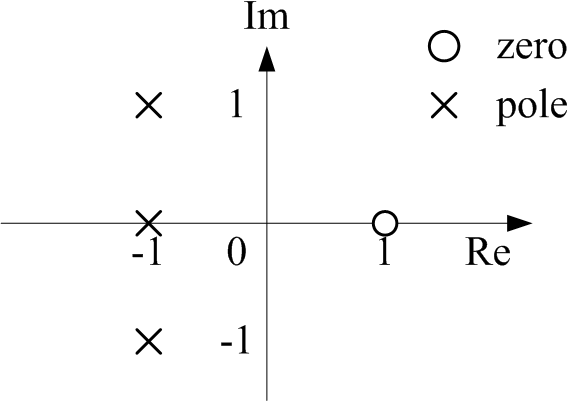
\includegraphics[height=3.5cm]{8.1.3-1.png}
\end{figure}

%============================================================
\subsection{系统框图}

并联系统(parallel interconnection)
\begin{figure}[h]
\centering
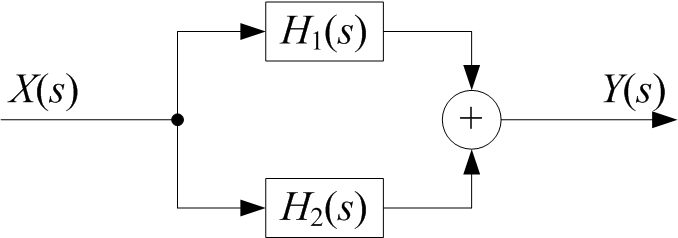
\includegraphics[height=2cm]{8.1.4-1.png}
\end{figure}
\[
H\left( s \right) =H_1\left( s \right) +H_2\left( s \right)
\]

串联系统(series interconnection),也称级联(cascade interconnection)
\begin{figure}[h]
\centering
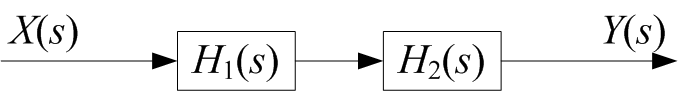
\includegraphics[height=0.8cm]{8.1.4-2.png}
\end{figure}
\[
H\left( s \right) =H_1\left( s \right) \cdot H_2\left( s \right)
\]

负反馈系统(negative feedback interconnection)
\begin{figure}[ht]
\centering
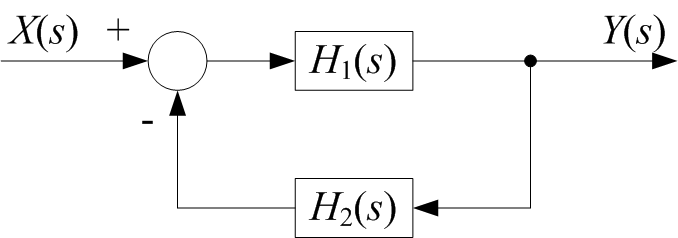
\includegraphics[height=2cm]{8.1.4-3.png}
\end{figure}
\[
H\left( s \right) =\frac{H_1\left( s \right)}{1+H_1\left( s \right) \cdot H_2\left( s \right)}
\]

%============================================================
\subsection{Python应用——scipy.signal中的传递函数类}

scipy.signal.lti()用零极点的方式生成传递函数类。
\begin{figure}[h]
\centering
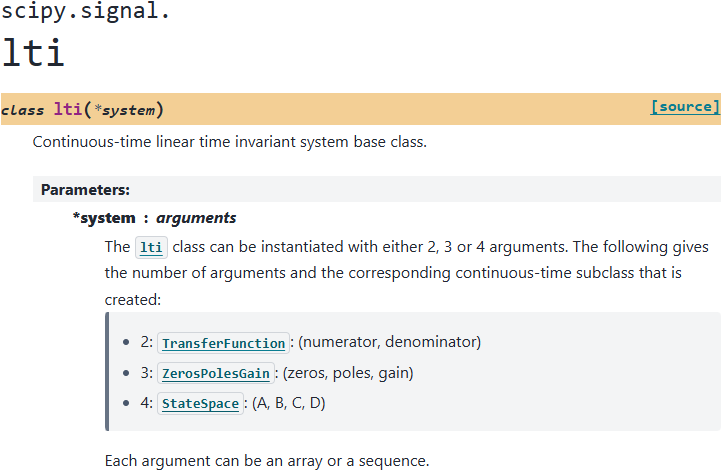
\includegraphics[width=8cm]{8.1.5-1.png}
\end{figure}

scipy.signal.TransferFunction()用多项式的方式生成传递函数类。
\begin{figure}[h]
\centering
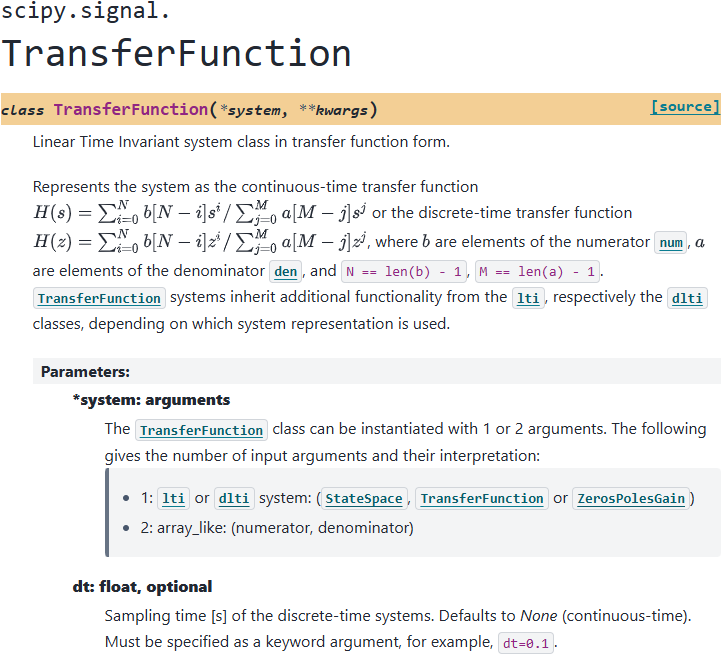
\includegraphics[width=8cm]{8.1.5-2.png}
\end{figure}

~

\begin{example}
\[
H\left( s \right) =\frac{5\left( s-1 \right) \left( s-2 \right)}{\left( s-3 \right) \left( s-4 \right)}
\]
\end{example}

\begin{python}
>>> scipy.signal.lti([1, 2], [3, 4], 5)
ZerosPolesGainContinuous(
array([1, 2]),
array([3, 4]),
5,
dt: None
)
\end{python}

~

\begin{example}
\[
H\left( s \right) =\frac{s^2+3s+4}{s^2+2s+1}
\]
\end{example}

\begin{python}
>>> num = [1,3,4]
>>> den = [1,2,1]
>>> scipy.signal.TransferFunction(num, den)
TransferFunctionContinuous(
array([1., 3., 4.]),
array([1., 2., 1.]),
dt: None
)
\end{python}

%============================================================
\subsection{电路中的传递函数}

\begin{tcolorbox}
很多情况下,我们不需要通过微分方程获得系统传递函数。
而是通过分析构成系统的组件的时域表达式,将其转换为s域表达式,然后根据组件之间的串并联及反馈的拓扑关系直接写出传递函数。
\end{tcolorbox}

以电路为例,首先将基本元器件(电阻、电容、电感)的电压电流关系式两端分别作LT,得到它们的s域表达式:
\[
\begin{array}{l}
	u\left( t \right) =Ri\left( t \right)\\
	\frac{du\left( t \right)}{dt}=\frac{1}{C}i\left( t \right)\\
	u\left( t \right) =L\frac{di\left( t \right)}{dt}\\
\end{array}\overset{\mathscr{L}}{\longleftrightarrow}\begin{array}{l}
	U\left( s \right) =RI\left( s \right)\\
	U\left( s \right) =\frac{1}{sC}I\left( s \right) +\frac{1}{s}u\left( 0 \right)\\
	U\left( s \right) =sLI\left( s \right) -Li\left( 0 \right)\\
\end{array}
\]
\begin{itemize}
    \item $u\left( t \right) ,i\left( t \right) $:元件两端电压,流经元件的电流;
    \item $U\left( s \right) ,I\left( s \right) $:$u\left( t \right) ,i\left( t \right) $的LT;
    \item $u\left( 0 \right) $:电容的初始电压;
    \item $i\left( 0 \right) $:电感的初始电流。
\end{itemize}
特别地,当电路系统无初始储能时(电容无储电,电感无磁能),它们的s域表达式为:
\[
\begin{array}{l}
	u\left( t \right) =Ri\left( t \right)\\
	\frac{du\left( t \right)}{dt}=\frac{1}{C}i\left( t \right)\\
	u\left( t \right) =L\frac{di\left( t \right)}{dt}\\
\end{array}\overset{\mathscr{L}}{\longleftrightarrow}\begin{array}{l}
	U\left( s \right) =RI\left( s \right)\\
	U\left( s \right) =\frac{1}{sC}I\left( s \right)\\
	U\left( s \right) =sLI\left( s \right)\\
\end{array}
\]
由于这三类元器件组成的系统为因果的LTI系统,符合传递函数的串并联定理,所以由电阻、电容、电感在s域可以视为“普通的”线性元件从而进行串并联。

也可以认为基尔霍夫定律在s域也是成立的。

~

\begin{example}
以RC电路例,假设电路零状态,$x\left( t \right) =1\mathrm{V},R=1\Omega ,C=1\mathrm{F}$,计算系统在0~10S这段时间内的输出。
\begin{figure}[h]
\centering
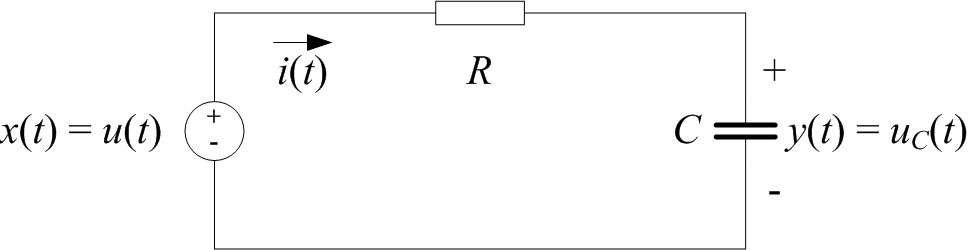
\includegraphics[height=2cm]{1.5.1-1.png}
\end{figure}
\end{example}

系统传递函数:
\[
H\left( s \right) =\frac{\frac{1}{sC}}{R+\frac{1}{sC}}=\frac{1}{sRC+1}=\frac{1}{s+1}
\]
输入$x\left( t \right) =1\mathrm{V}$视为单位阶跃信号,用Scipy库的signal模块的step()函数可以画出系统对单位阶跃信号的时域响应。

\begin{python}
H    = signal.lti([1],[1,1])
t, y = signal.step(H, T=np.arange(0,10,0.1))

ax.plot(t, y)
\end{python}

\begin{figure}[h]
\centering
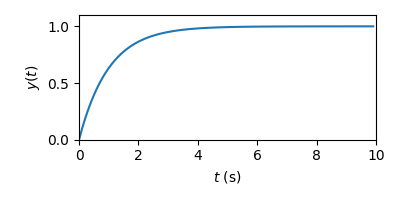
\includegraphics[height=3cm]{8.1.6-1.png}
\end{figure}

~

\begin{example}
如下电路,设输入为电压源电压,输出为流经电容$C_1$的电流,求系统的传递函数。
\begin{figure}[ht]
\centering
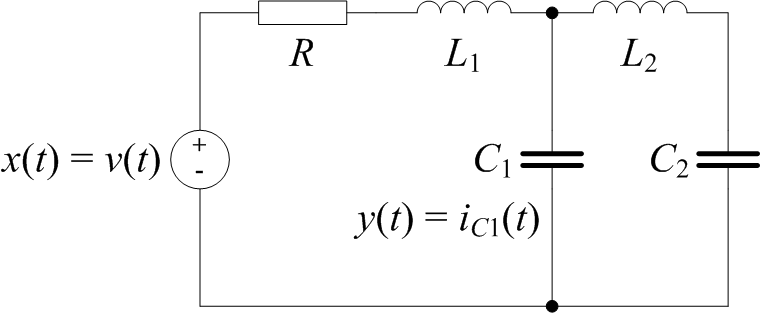
\includegraphics[height=2.5cm]{8.1.6-2.png}
\end{figure}
\end{example}

假设$C_1$的电压的LT为$U\left( s \right) $,有:
\begin{align*}
&\because Y\left( s \right) =\frac{V\left( s \right)}{1/sC_1}=\frac{\left( sL_2+1/sC_2 \right) \parallel 1/sC_1}{R+sL_1+\left( sL_2+1/sC_2 \right) \parallel 1/sC_1}X\left( s \right) \cdot sC_1 \\
&\therefore H\left( s \right) =\frac{\left( sL_2+\frac{1}{sC_2} \right) \parallel \frac{1}{sC_1}}{R+sL_1+\left( sL_2+\frac{1}{sC_2} \right) \parallel \frac{1}{sC_1}}\cdot sC_1
\end{align*}




